\subsection{Problem Formulation}
We use TVM~\cite{Chen18} to investigate the performance of matrix tiling for GEMM. TVM facilitates tiling optimization by generating Intermediate Representation (IR) of a particular configuration. Fig.~\ref{fig:gemm_ir} is a simple example IR of GEMM tiling configuration with a blocking factor of 32 on x86 CPU for GEMM with $(m=1024, k=1024, n=1024)$ (short as $(1024,1024,1024)$).
\begin{figure}[htb]
    \centering
    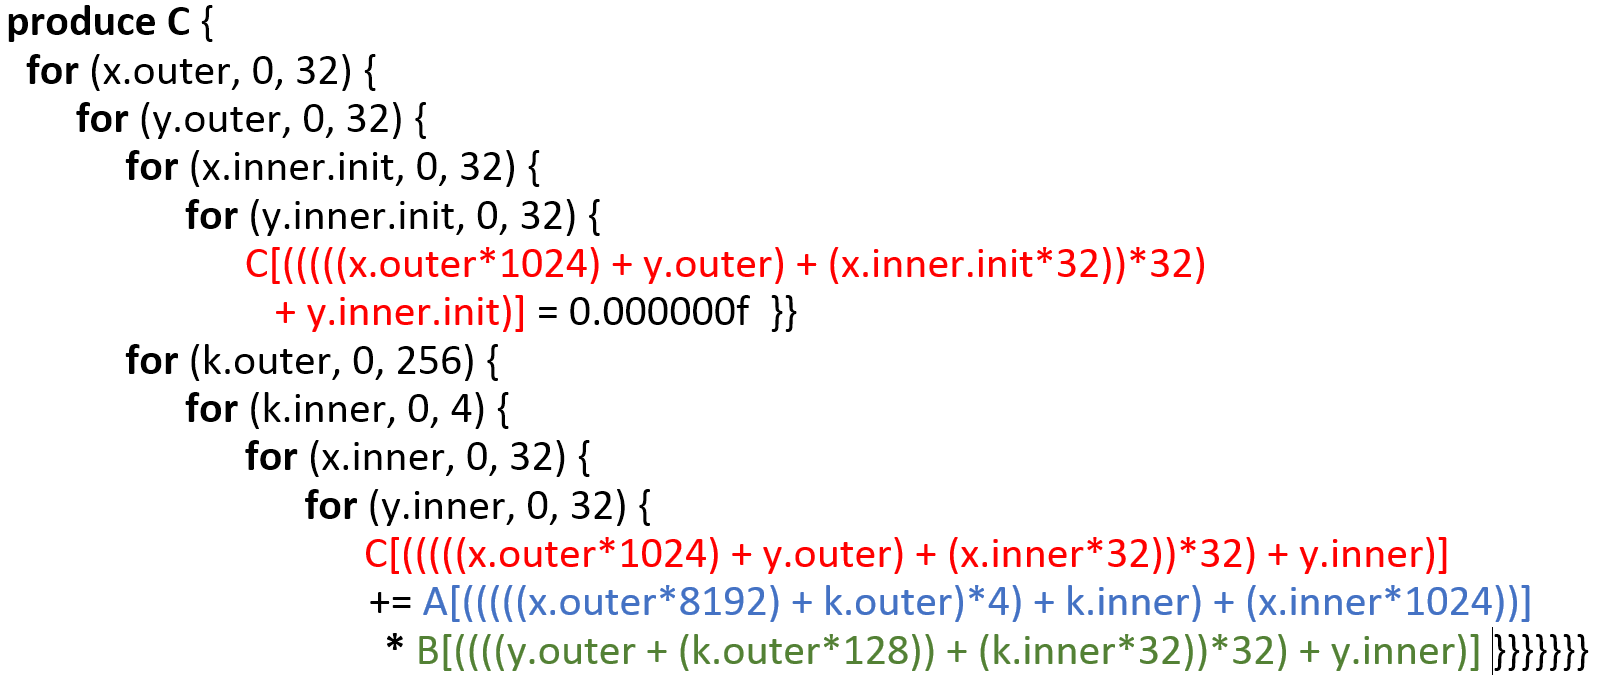
\includegraphics[width=3in]{3_GEMM_backgrounds/gemm_ir.png}
    \caption{IR of GEMM with a blocking factor of 32}
    \label{fig:gemm_ir}
\end{figure}

% \begin{definition}
\noindent
\textbf{Definition:}
Generally, a GEMM tiling configuration can be defined as 
\begin{equation}
    \overrightarrow{\xi} = \overrightarrow{\xi_m} \times \overrightarrow{\xi_k} \times \overrightarrow{\xi_n},
\end{equation}
where
\begin{equation}
     \overrightarrow{\xi_m} =\{ \left[m_0,\ldots,m_i, \ldots m_{d_m-1} \right] |  \Pi_{i=0}^{d_m-1} m_i=m \},
\end{equation}
\begin{equation}
     \overrightarrow{\xi_k} =\{ \left[k_0,\ldots,k_l, \ldots k_{d_k-1} \right] |  \Pi_{l=0}^{d_k-1} k_l=k \},
\end{equation}
\begin{equation}
     \overrightarrow{\xi_n} =\{ \left[n_0,\ldots,n_j, \ldots n_{d_n-1} \right] |  \Pi_{j=0}^{d_n-1} n_j=n \}.
\end{equation}
% \end{definition}
Multiplication of two matrices $A(m\times k)$ and $B(k\times n)$ produces matrix $C(m\times n)$. $d_m$, $d_k$ and $d_n$ are the number of nested loops for each dimension $m$, $k$ and $n$, respectively.  $m_i, k_l, n_j$, $\forall i \in [0, d_m)$ $\forall l \in [0, d_k)$ $\forall j \in [0, d_n)$, are the number of iterations of a respective loop. The configuration in Fig.~\ref{fig:gemm_ir} is $m_0=m_1=32$, $k_0=256, k_1=4$, $n_0=n_1=32$, and $d_m=d_k=d_n=2$.

Constrained by the definition of tiling configuration, we can formulate the following optimization problem:
\begin{equation}\nonumber
    \begin{array}{l}
       \mathop {\min }\limits_{s} T_{cost}(s ; m,k,n,d_m,d_k,d_n).
    \end{array}
\end{equation}
The objective function of this problem is to find an optimal tiling configuration that has minimal running time on target hardware. $T_{cost}$ denotes the running time for the configuration $s$, given the dimension of matrices as $m,k,n$ and the number of the nested loops on each dimension as $d_m, d_k, d_n$. 

%In our experiments, we run GEMM tiling configurations on Nivida CUDA GPU, more specifically $d_m=4$, $d_k=2$ and $d_n=4$.